\documentclass[11pt]{amsart}
\usepackage{geometry}                % See geometry.pdf to learn the layout options. There are lots.
\geometry{letterpaper}                   % ... or a4paper or a5paper or ... 
%\geometry{landscape}                % Activate for for rotated page geometry
\usepackage[parfill]{parskip}    % Activate to begin paragraphs with an empty line rather than an indent
\usepackage{graphicx}
\usepackage{amssymb}
\usepackage{epstopdf}
\usepackage{amsmath}
\DeclareGraphicsRule{.tif}{png}{.png}{`convert #1 `dirname #1`/`basename #1 .tif`.png}

%---------------------Listings Package--------------------%
\usepackage{listings}
\usepackage{color}
\definecolor{mygreen}{rgb}{0,0.6,0}
\definecolor{mygray}{rgb}{0.5,0.5,0.5}
\definecolor{mymauve}{rgb}{0.58,0,0.82}
\lstset{ %
  backgroundcolor=\color{white},   % choose the background color; you must add \usepackage{color} or \usepackage{xcolor}
  basicstyle=\footnotesize,        % the size of the fonts that are used for the code
  breakatwhitespace=flase,         % sets if automatic breaks should only happen at whitespace
  breaklines=false,                 % sets automatic line breaking
  captionpos=b,                    % sets the caption-position to bottom
  commentstyle=\color{mygreen},    % comment style
  deletekeywords={...},            % if you want to delete keywords from the given language
  escapeinside={\%*}{*)},          % if you want to add LaTeX within your code
  extendedchars=true,              % lets you use non-ASCII characters; for 8-bits encodings only, does not work with UTF-8
  frame=single,	                   % adds a frame around the code
  keepspaces=true,                 % keeps spaces in text, useful for keeping indentation of code (possibly needs columns=flexible)
  keywordstyle=\color{blue},       % keyword style
  language=Octave,                 % the language of the code
  otherkeywords={*,...},           % if you want to add more keywords to the set
  numbers=left,                    % where to put the line-numbers; possible values are (none, left, right)
  numbersep=5pt,                   % how far the line-numbers are from the code
  numberstyle=\tiny\color{mygray}, % the style that is used for the line-numbers
  rulecolor=\color{black},         % if not set, the frame-color may be changed on line-breaks within not-black text (e.g. comments (green here))
  showspaces=false,                % show spaces everywhere adding particular underscores; it overrides 'showstringspaces'
  showstringspaces=false,          % underline spaces within strings only
  showtabs=false,                  % show tabs within strings adding particular underscores
  stepnumber=2,                    % the step between two line-numbers. If it's 1, each line will be numbered
  stringstyle=\color{mymauve},     % string literal style
  tabsize=2,	                   % sets default tabsize to 2 spaces
  title=\lstname                   % show the filename of files included with \lstinputlisting; also try caption instead of title
}
%-----------------------------------------------------------------%


%-------------------Landscape Package------------------%
\usepackage{pdflscape}
%-----------------------------------------------------------------%

\title{Numerical Methods\\[0.1in]
	ECSE 543 - Assignment 2}
\author{Mido Assran - 260505216}
\date{\today}

\begin{document}
\maketitle

\section*{Question 1}
\vspace*{-0.2in}
\noindent\rule{\textwidth}{0.4pt}

The goal is to find the disjoint local \textbf{S}-matrix for each finite element triangle, and subsequently find the global conjoint \textbf{S}-matrix for the finite difference mesh composed of the triangular finite elements.

\begin{figure}[h]
    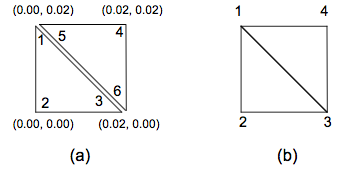
\includegraphics[width=0.6\textwidth]{assets/question_1.png}
    \caption{a) Disjoint finite elements with local numbering and vertex coordinates $(x,y)$ in meters b) Conjoint finite element mesh with global numbering}
    \label{fig:q1_mesh}
\end{figure}

The first step to finding the disjoint local \textbf{S}-matrix of each finite element triangle is to find the potentials in the elements. We take the potential, $U$, to vary linearly over the $(x,y)$ plane - note that the assumption of a linearly varying potential within the triangular element is equivalent to assuming that the electric field is uniform within the element (this is a good assumption in parallel-plate conductor type settings). Equation (\ref{eq:q1_potential}) shows the general linear relationship for the potential - constants $a$, $b$, and $c$ are to be determined.

\begin{equation}
	\label{eq:q1_potential}
	U = a + bx + cy
\end{equation}

Denoting the potentials at the vertices by $U_v$, where v is the vertex number set by the local ordering, we can solve the linear system of equations shown in equation (\ref{eq:q1_constants}) for the constants $a$, $b$, and $c$ where the potential at local vertex $v$ has coordinates given by $(x_v,y_v)$.

\begin{equation}
	\label{eq:q1_constants}
        \begin{bmatrix}
            U_1\\
            U_2\\
            U_3
        \end{bmatrix}
        =
        \begin{bmatrix}
            1 & x_1 & y_1\\ 
            1 & x_2 & y_2\\ 
            1 & x_3 & y_3 
        \end{bmatrix} 
        \begin{bmatrix}
            a\\
            b\\
            c
        \end{bmatrix}
\end{equation}

To solve for the constants we have the closed form relationship shown in equation (\ref{eq:q1_constants_closed_form}), where $adj$ is used to denote the adjugate of the matrix (found by taking the transpose of its cofactor matrix), and $det$ its determinant.

\begin{equation}
	\label{eq:q1_constants_closed_form}
        \begin{bmatrix}
            a\\
            b\\
            c
        \end{bmatrix}
        =
        \frac{
        	   adj
            \begin{bmatrix}
                1 & x_1 & y_1\\ 
                1 & x_2 & y_2\\ 
                1 & x_3 & y_3 
            \end{bmatrix}
            }{
            det
            \begin{bmatrix}
                1 & x_1 & y_1\\ 
                1 & x_2 & y_2\\ 
                1 & x_3 & y_3 
            \end{bmatrix}
        }
         \begin{bmatrix}
            U_1\\
            U_2\\
            U_3
        \end{bmatrix}
\end{equation}

The result of equation (\ref{eq:q1_constants_closed_form}) gives us the constants in terms of the vertex potentials as shown in equation (\ref{eq:q1_solved_cosntants}), where $A_e$ is used to denote the area of the triangular finite element $e$.

\begin{equation}
	\label{eq:q1_solved_cosntants}
        \begin{bmatrix}
            a\\
            b\\
            c
        \end{bmatrix}
        =
        \frac{
            \begin{bmatrix}
                (x_2y_3 - x_3y_2) & (x_3y_1 - x_1y_3) & (x_1y_2 - x_2y_1)\\ 
                (y_2 - y_3) & (y_3 - y_1) & (y_1 - y_2)\\ 
                (x_3 - x_2) & (x_1 - x_3) & (x_2 - x_1) 
            \end{bmatrix}
            }{
            2A_e
        	    }
         \begin{bmatrix}
            U_1\\
            U_2\\
            U_3
        \end{bmatrix}
\end{equation}

Since the potential in equation (\ref{eq:q1_potential}) can be written as 
$$ U =  
        \begin{bmatrix}
            1 & x & y
        \end{bmatrix}
	\begin{bmatrix}
            a\\
            b\\
            c
        \end{bmatrix}
$$

then we can directly substitute equation (\ref{eq:q1_solved_cosntants}) into the above representation and rewrite the potential as: $$ U = \sum^{3}_{i=1} \alpha_i(x,y) U_i$$

where the $\alpha_i(x,y)$ (also known as the linear interpolation functions) are given by equations (\ref{eq:q1_interpolation_functions_1}), (\ref{eq:q1_interpolation_functions_2}), and (\ref{eq:q1_interpolation_functions_3}),

\begin{equation}
    \label{eq:q1_interpolation_functions_1}
    \alpha_1 = \frac{1}{2A_e}[(x_2y_3 - x_3y_2) + (y_2 - y_3)x + (x_3 - x_2)y]
\end{equation}
\begin{equation}
    \label{eq:q1_interpolation_functions_2}
    \alpha_1 = \frac{1}{2A_e}[(x_3y_1 - x_1y_3) + (y_3 - y_1)x + (x_1 - x_3)y]
\end{equation}
\begin{equation}
    \label{eq:q1_interpolation_functions_3}
    \alpha_1 = \frac{1}{2A_e}[(x_1y_2 - x_2y_1) + (y_1 - y_2)x + (x_2 - x_1)y]
\end{equation}

and $A_e$ is given by equation (\ref{eq:q1_area}).

\begin{equation}
    \label{eq:q1_area}
    A_e = \frac{1}{2}[(x_2y_3 - x_3y_2) + (x_3y_1 - x_1y_3) + (x_1y_2 - x_2y_1)]
\end{equation}


The energy in each finite element is given by equation (\ref{eq:q1_energy}), where $W^{(e)}$ is the energy per unit length associated with finite element $e$, $U$ is the potential - which in general will vary with coordinates $(x,y)$ as was already established, and the integral is swept over $A_e$, which is the area occupied by element $e$. \footnotesize{*Note that there the permittivity of the medium is neglected in the equation}.
\begin{equation}
	\label{eq:q1_energy}
	W^{(e)} = \frac{1}{2} \int_{A_e}| \nabla U|^2 dS
\end{equation}

Equations (\ref{eq:q1_energy_2}), and (\ref{eq:q1_energy_3}) are derived by just making a simple substitution for $U$ in equation (\ref{eq:q1_energy}) using the derived series representation in terms of the interpolation functions and vertex potentials.

\begin{equation}
	\label{eq:q1_energy_2}
	W^{(e)} = \frac{1}{2}\sum^{3}_{i=1}\sum^{3}_{j=1}U_{i}\left[ \int_{A_e} \nabla \alpha_i \bullet \nabla \alpha_j dS \right]U_{j}
\end{equation}
\begin{equation}
	\label{eq:q1_energy_3}
	W^{(e)} = \frac{1}{2} U^T S^{(e)} U
\end{equation}

Finally we are able to determine the local $S^{(e)}$ depicted in equation (\ref{eq:q1_energy_3}), whose entries are given by equation (\ref{eq:q1_local_s}).

\begin{equation}
	\label{eq:q1_local_s}
	S^{(e)}_{(i,j)} = \int_{A_e} \nabla \alpha_i \bullet \nabla \alpha_j dS
\end{equation}

Therefore we have:

\begin{equation}
	\label{eq:q1_local_s11}
	S^{(e)}_{(1,1)} = \frac{1}{4A}[(y_2-y_3)^2 + (x_3 - x_2)^2]
\end{equation}
\begin{equation}
	\label{eq:q1_local_s12}
	S^{(e)}_{(1,2)} = \frac{1}{4A}[(y_2-y_3)(y_3 - y_1) + (x_3 - x_2)(x_1 - x_3)]
\end{equation}
\begin{equation}
	\label{eq:q1_local_s13}
	S^{(e)}_{(1,3)} = \frac{1}{4A}[(y_2-y_3)(y_1 - y_2) + (x_3 - x_2)(x_2 - x_1)]
\end{equation}
\begin{equation}
	\label{eq:q1_local_s22}
	S^{(e)}_{(2,2)} = \frac{1}{4A}[(y_3 - y_1)^2 + (x_1 - x_3)^2]
\end{equation}
\begin{equation}
	\label{eq:q1_local_s23}
	S^{(e)}_{(2,3)} = \frac{1}{4A}[(y_3 - y_1)(y_1 - y_2) + (x_1 - x_3)(x_2 - x_1)]
\end{equation}
\begin{equation}
	\label{eq:q1_local_s33}
	S^{(e)}_{(3,3)} = \frac{1}{4A}[(y_1 - y_2)^2 + (x_2 - x_1)^2]
\end{equation}
\begin{equation}
	\label{eq:q1_local_s_symmetry}
	S^{(e)}_{(1,2)} = S^{(e)}_{(2,1)}, \quad S^{(e)}_{(3,1)} = S^{(e)}_{(1,3)}, \quad S^{(e)}_{(3,2)} = S^{(e)}_{(2,3)}
\end{equation}

Letting $S^{(L)}$ represent the disjoint matrix for the lower triangular element in Figure \ref{fig:q1_mesh}.a, and $S^{(U)}$ represent the disjoint matrix for the upper triangular element in Figure \ref{fig:q1_mesh}.b, we can apply some \textit{plug-and-chug} to solve for the matrix entries where the local numberings relative to the derived equations are created in a counterclockwise fashion. The coordinates for the vertices in each element are:\\

\begin{center}
    \begin{tabular}{ c c } 
    $S^{(L)}$ & \\
    \hline
     $(x1,y1):$ & $(0,00, 0.02)$ \\ 
     $(x2,y2):$ & $(0.00, 0.00)$ \\ 
     $(x3,y3):$ & $(0.02, 0.00)$ \\[0.2in]
     $S^{(U)}$ & \\
     \hline
     $(x1,y1):$ & $(0.02, 0.02)$ \\ 
     $(x2,y2):$ & $(0.00, 0.02)$ \\ 
     $(x3,y3):$ & $(0.02, 0.00)$ \\ 

\end{tabular}
\end{center}

We have $A_e = \frac{1}{2}[(0.02 \cdot 0.02)] = 0.0002$, which is identical for $e = L$ and $e = U$.

$$
	S^{(L)}_{(1,1)} = \frac{1}{4(0.0002)}[(0.02)^2]
$$$$
	S^{(L)}_{(1,2)} = \frac{1}{4(0.0002)}[(0.02)(-0.02)]
$$$$
	S^{(L)}_{(1,3)} = \frac{1}{4(0.0002)}[0]
$$$$
	S^{(L)}_{(2,2)} = \frac{1}{4(0.0002)}[(-0.02)^2 + (-0.02)^2]
$$$$
	S^{(L)}_{(2,3)} = \frac{1}{4(0.0002)}[(-0.02)(0.02)]
$$$$
	S^{(L)}_{(3,3)} = \frac{1}{4(0.0002)}[(0.02)^2]
$$$$
	S^{(L)}_{(1,2)} = S^{(L)}_{(2,1)}, \quad S^{(L)}_{(3,1)} = S^{(L)}_{(1,3)}, \quad S^{(L)}_{(3,2)} = S^{(L)}_{(2,3)}
$$

\begin{center}
\boxed{
	S^{(L)} = 
            \begin{bmatrix}
            0.5 & -0.5 & 0\\
            -0.5 & 1 & -0.5\\
            0 & -0.5 & 0.5
            \end{bmatrix}
}
\end{center}

$$
	S^{(U)}_{(1,1)} = \frac{1}{4(0.0002)}[(0.02)^2 + (0.02)^2]
$$$$
	S^{(U)}_{(1,2)} = \frac{1}{4(0.0002)}[(0.02)(-0.02)]
$$$$
	S^{(U)}_{(1,3)} = \frac{1}{4(0.0002)}[(0.02)(-0.02)]
$$$$
	S^{(U)}_{(2,2)} = \frac{1}{4(0.0002)}[(-0.02)^2]
$$$$
	S^{(U)}_{(2,3)} = \frac{1}{4(0.0002)}[0]
$$$$
	S^{(U)}_{(3,3)} = \frac{1}{4(0.0002)}[(-0.02)^2]
$$$$
	S^{(U)}_{(1,2)} = S^{(U)}_{(2,1)}, \quad S^{(U)}_{(3,1)} = S^{(U)}_{(1,3)}, \quad S^{(U)}_{(3,2)} = S^{U}_{(2,3)}
$$

\begin{center}
\boxed{
	S^{(U)} = 
            \begin{bmatrix}
            1 & -0.5 & -0.5\\
            -0.5 & 0.5 & 0\\
            -0.5 & 0 & 0.5
            \end{bmatrix}
}
\end{center}

The global conjoint \textbf{S}-matrix can be found using the disjoint finite element $S^{(e)}$ matrices. The energy of the entire finite element mesh is found by summing the energies of each individual element as is shown in equation (\ref{eq:q1_energy_mesh}).

\begin{equation}
	\label{eq:q1_energy_mesh}
	W = \sum_{L, U} W^{(e)} = \frac{1}{2} U^{T}_{dis} S_{dis} U_{dis}
\end{equation}

where $$ S_{dis} = \begin{bmatrix} S^{(L)} & \\ & S^{(U)}\end{bmatrix} =
\begin{bmatrix}
            0.5 & -0.5 & 0 & 0 & 0 & 0\\
            -0.5 & 1 & -0.5 & 0 & 0 & 0\\
            0 & -0.5 & 0.5 & 0 & 0 & 0\\
            0 & 0 & 0 & 1 & -0.5 & -0.5\\
            0 & 0 & 0 & -0.5 & 0.5 & 0\\
            0 & 0 & 0 & -0.5 & 0 & 0.5
\end{bmatrix}
$$.

Substituting $U_{dis} = C U_{con}$ (whose relationship is shown in equation (\ref{eq:q1_potentials_con_dis})) into equation (\ref{eq:q1_energy_mesh}), gives $$W = \frac{1}{2} U^{T}_{con} C^{T} S_{dis} C U_{con}$$

where $S = C^{T} S_{dis} C$

\begin{equation}
	\label{eq:q1_potentials_con_dis}
        \begin{bmatrix}
            U_1\\
            U_2\\
            U_3\\
            U_4\\
            U_5\\
            U_6\\
        \end{bmatrix}_{dis}
        =
        \begin{bmatrix}
	1 & 0 & 0 & 0\\
	0 & 1 & 0 & 0\\
	0 & 0 & 1 & 0\\
	0 & 0 & 0 & 1\\
	1 & 0 & 0 & 0\\
	0 & 0 & 1 & 0
        \end{bmatrix}
        \begin{bmatrix}
            U_1\\
            U_2\\
            U_3\\
            U_4
        \end{bmatrix}_{conj}
\end{equation}

therefore 
$$C =         \begin{bmatrix}
                    	1 & 0 & 0 & 0\\
                    	0 & 1 & 0 & 0\\
                    	0 & 0 & 1 & 0\\
                    	0 & 0 & 0 & 1\\
                    	1 & 0 & 0 & 0\\
                    	0 & 0 & 1 & 0
                \end{bmatrix}
$$

Carrying out the matrix multiplication we have the following for the global \textbf{S}-matrix (which was computed using MATLAB).

\begin{figure}[h]
    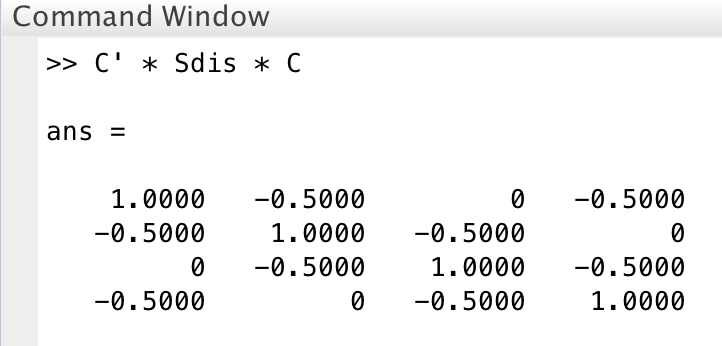
\includegraphics[width=0.5\textwidth]{assets/question_1_matlab.png}
    \caption{MATLAB computation of the global \textbf{S}-matrix}
    \label{fig:q1_matlab}
\end{figure}

\vspace{0.25in}
\begin{center}
\boxed{
	S = 
            \begin{bmatrix}
                1 & -0.5 & 0 & -0.5\\
                -0.5 & 1 & -0.5 & 0\\
                0 & -0.5 & 1 & -0.5\\
                -0.5 & 0 & -0.5 & 1\\
            \end{bmatrix}
}
\end{center}

\pagebreak

\section*{Question 2}
\vspace*{-0.2in}
\noindent\rule{\textwidth}{0.4pt}

\subsection*{Part a}
Using the two-element mesh shown in Figure \ref{fig:q1_mesh} as a building block, a finite element mesh is constructed for one-quarter of the cross-section of the coaxial cable shown in Figure \ref{fig:q2_coax}. The equivalent one-quarter mesh is shown in Figure \ref{fig:q2_mesh}. \textbf{To simplify the node coordinates in subsequent calculations, the x, y coordinates were renormalized to the bottom left corner of Figure \ref{fig:q2_mesh}}.

\begin{figure}[h]
    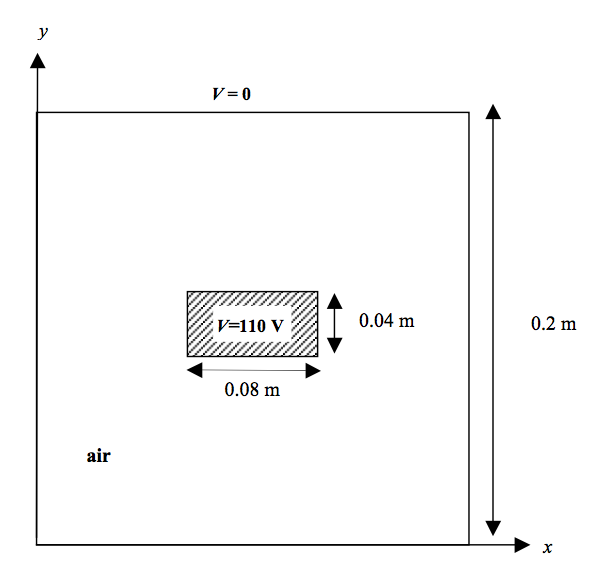
\includegraphics[width=0.35\textwidth]{assets/coax.png}
    \caption{Rectangular coax.}
    \label{fig:q2_coax}
\end{figure}

\begin{figure}[h]
    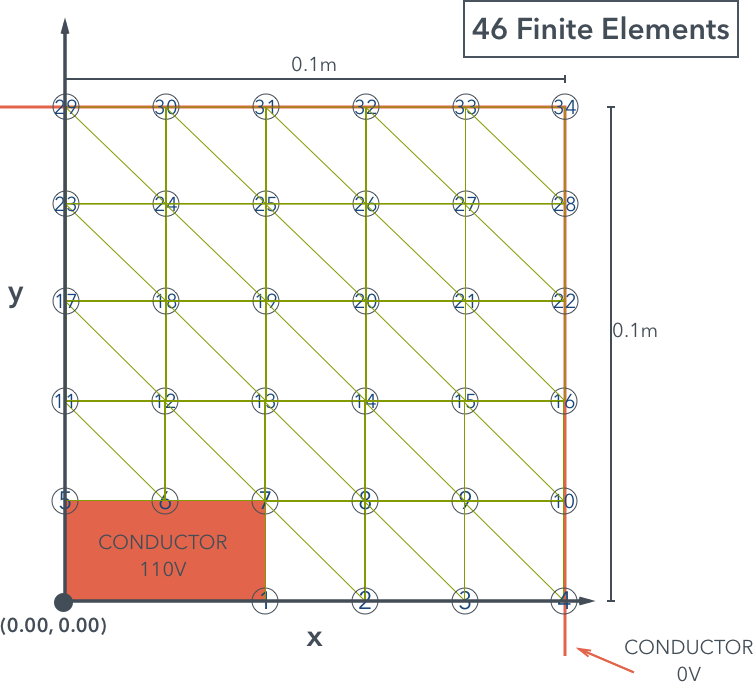
\includegraphics[width=0.6\textwidth]{assets/q2_mesh.png}
    \caption{Global ordering of a finite element mesh for one quarter of a coax.}
    \label{fig:q2_mesh}
\end{figure}

\begin{table}[t]
    \scriptsize
    \begin{tabular}[t]{c c c}
        	\textit{node.dat} & & \\ \hline
        1    &   0.04  &  0.00\\
        2    &   0.06  &  0.00\\
        3    &   0.08  &  0.00\\
        4    &   0.10  &  0.00\\
        5    &   0.00  &  0.02\\
        6    &   0.02  &  0.02\\
        7    &  0.04   & 0.02\\
        8    &   0.06  &  0.02\\
        9    &   0.08  &  0.02\\
        10  &   0.10  &  0.02\\
        11  &    0.00  &   0.04\\
        12  &    0.02  &   0.04\\
        13  &    0.04  &   0.04\\
        14  &    0.06  &  0.04\\
        15  &    0.08  &  0.04\\
        16  &    0.10  &  0.04\\
        17  &    0.00  &  0.06\\
        18  &    0.02  &  0.06\\
        19  &    0.04  &  0.06\\
        20  &    0.06  &  0.06\\
        21  &    0.08  &  0.06\\
        22  &    0.10  &  0.06\\
        23  &    0.00  &  0.08\\
        24  &    0.02  &  0.08\\
        25  &    0.04  &  0.08\\
        26  &    0.06  &  0.08\\
        27  &    0.08  &  0.08\\
        28  &    0.10  &  0.08\\
        29  &    0.00  &  0.10\\
        30  &    0.02  &  0.10\\
        31  &    0.04  &  0.10\\
        32  &    0.06  &  0.10\\
        33  &    0.08  &  0.10\\
        34  &    0.10  &  0.10
    \end{tabular}
    \hfill
    \begin{tabular}[t]{c c}
        	\textit{bc.dat} & \\ \hline
	5    &   110.0\\
        6     &   110.0\\
        7     &   110.0\\
        4     &   0.0\\
        10   &    0.0\\
        16   &    0.0\\
        22   &    0.0\\
        28   &    0.0\\
        34   &    0.0\\
        33   &    0.0\\
        32   &    0.0\\
        31   &   0.0\\
        30   &   0.0\\
        29   &   0.0
    \end{tabular}
    \hfill
    \begin{tabular}[t]{c c c c}
    	\textit{tri.dat} & & & \\ \hline
        1    &   2   &    7 &0\\
        2    &   8   &    7 &0\\
        2    &   3   &    8 &0\\
        3    &   9   &    8 &0\\
        3    &   4   &    9 &0\\
        4    &   10 &    9 &0\\
        5    &   6   &    11 &0\\
        6    &   12 &    11 &0\\
        6    &   7   &    12 &0\\
        7    &   13 &    12 &0\\
        7    &   8   &    12 &0\\
        8    &   14 &    13 &0\\
        8    &   9   &    14 &0\\
        9    &   15 &     14 &0\\
        9    &   10 &     15 &0\\
        10  &    16&     15 &0\\
        11  &    12&     17 &0\\
        12  &    18&     17 &0\\
        12  &    13&     18 &0\\
        13  &    19&     18 &0\\
        13  &    14&     19 &0\\
        14  &    20&     19 &0\\
        14  &    15&     20 &0\\
        15  &    21&     20 &0\\
        15  &    16&     21 &0\\
        16  &    22&     21 &0\\
        17  &    18 &    23 &0\\
        18  &    24&     23 &0\\
        18  &    19&     24 &0\\
        19  &    25&     24 &0\\
        19  &    20&     25 &0\\
        20  &    26&     25 &0\\
        20  &    21&     26 &0\\
        21  &    27&     26 &0\\
        21  &    22&     27 &0\\
        22  &    28&     27 &0\\
        23  &    24&     29 &0\\
        24  &    30&     29 &0\\
        24  &    25&     30 &0\\
        25  &    30&     31 &0\\
        25  &    26&     31 &0\\
        26  &    32&     31 &0\\
        26  &    27&     32 &0\\
        27  &    33&     32 &0\\
        27  &    28&     33 &0\\
        28  &    34&     33 &0\\        
    \end{tabular}
    \caption{SIMPLE2D input consisting of node coordinates, boundary conditions, and finite element vertex definitions from left to right}
    \label{tb:input}
\end{table}

The input file used for the SIMPLE2D Matlab program was split up into three files, \textit{node.dat}, \textit{bc.dat}, \textit{tri.dat}, which are shown in Table \ref{tb:input}. The \textit{node.dat} table lists the node numbers (according to the global ordering shown in Figure \ref{fig:q2_mesh}) and their respective x, y coordinates; the \textit{bc.dat} file lists the boundary nodes (according to the global ordering), and their respective potentials in Volts; lastly the \textit{tri.dat} table lists the nodes (according to the global ordering) that make up each triangular finite element with a zero terminated column. The data was split up for convenience of comprehension, however could've just as easily been stacked in a single file.

\subsection*{Part b}
The electrostatic potential solution was computed using the SIMPLE2D program with the mesh shown in Table \ref{tb:input}. The screenshot from the Matlab output is shown in Figure \ref{fig:q2_potentials} - \textbf{note that the coordinates shown in the Matlab output correspond to the renormalized x, y problem coordinates}. From the output, we deduce that by symmetry of the problem, the potential at point  (0.06, 0.04) is equivalent to the potential at node 19 in Figure \ref{fig:q2_mesh}. \textbf{The potential at (0.06, 0.04) is 41.4710 Volts}.

\begin{figure}[h]
    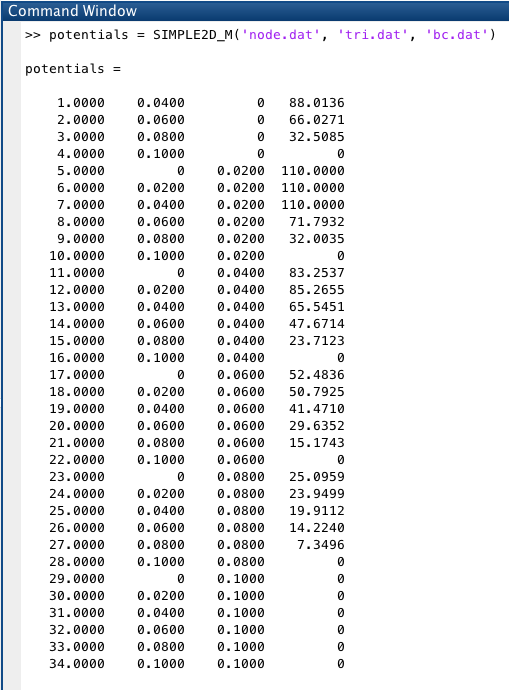
\includegraphics[width=0.6\textwidth]{assets/q2_potentials}
    \caption{SIMPLE2D Matlab output for the quarter-coax finite element mesh with renormalized x, y coordinates.}
    \label{fig:q2_potentials}
\end{figure}

\pagebreak

\subsection*{Part c}
To compute the capacitance per unit length obtained from the solution of the SIMPLE2D program, we start off by finding the energy per unit length contained in a square made up of two triangular finite elements:
$$ W = \frac{1}{2} \epsilon_{0} U^{T}_{con} S U_{con} $$
where the global S matrix is that found in \textit{Question 1}, and $U_{con}$ represents the vector of conjoint potentials according to the global ordering. After finding the energy in every micro-grid of the free-node problem domain (\textbf{not including the fixed potential domain}). We then sum up all of those energies, and multiply by 4 to obtain the energy per unit length in the entire free-space of the coax $ W^{(total)} = 4 * \sum_{q} W$. We then use
$$ W^{(total)} = \frac{1}{2} CV^2 $$
where C is the capacitance per unit length, and V is the potential difference across the coax (V = 110 Volts - 0 Volts in this case). The Matlab script used to carry out the above procedure is shown in Listing \ref{lstng:capacitance_pul} - again this Matlab script is based on the specific global ordering of Figure \ref{fig:q2_mesh}.
\lstinputlisting[language=Matlab, label=lstng:capacitance_pul, frame=single, caption=capacitance\_pul.m]{../capacitance_pul.m}
\boxed{\textbf{The capacitance per unit length is: \quad\quad $5.2627e-11 \quad Farads/m$}}

\pagebreak

\section*{Question 3}
\vspace*{-0.2in}
\noindent\rule{\textwidth}{0.4pt}
The conjugate gradient method implementation provided in Listing \ref{lstng:conjugate_gradient} is used to construct the finite difference equation for a quadrant of the coax, and subsequently solve it. The output for h=0.02 is shown in Figure \ref{fig:q3_cg}. Note that the value for $h$ is inputed by the user in the conjugate gradient program, thereby making it very easy to simply try out the problem with different inter-element spacings.
\begin{figure}[h!]
    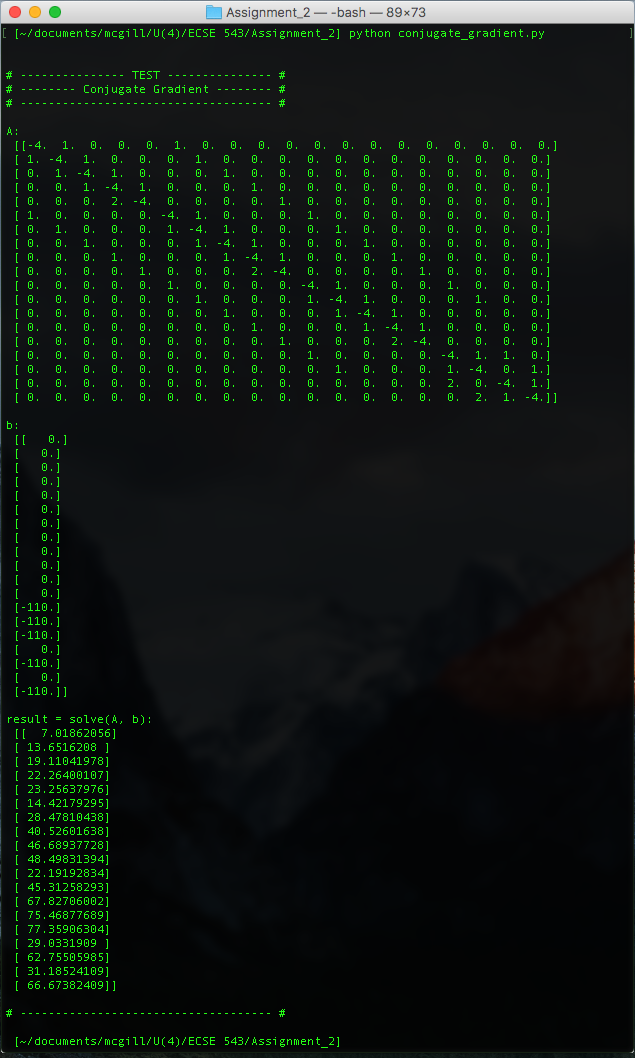
\includegraphics[width=0.6\textwidth]{assets/conjugate_gradient}
    \caption{Console output of conjugate gradient solver used to solve the unpreconditioned finite difference equation of the bottom-left quadrant of the coax}
    \label{fig:q3_cg}
\end{figure}

\pagebreak

\subsection*{Part a}
The finite difference matrix is tested using the choleski decomposition program written for Question 1 of Assignment 1 to ensure that it is positive definite. The choleski decomposition implementation is provided in Listing \ref{lstng:choleski} again for convenience. The console output is provided in Figure \ref{fig:q3_chol}. Unfortunately as it is, the matrix is NOT positive definite. To make it positive definite, we could precondition the finite difference system of equations with the transpose of the matrix. In other words instead of solving $Ax = b$, we could solve $HAx = Hb$ where $H=A^T$.
\begin{figure}[h!]
    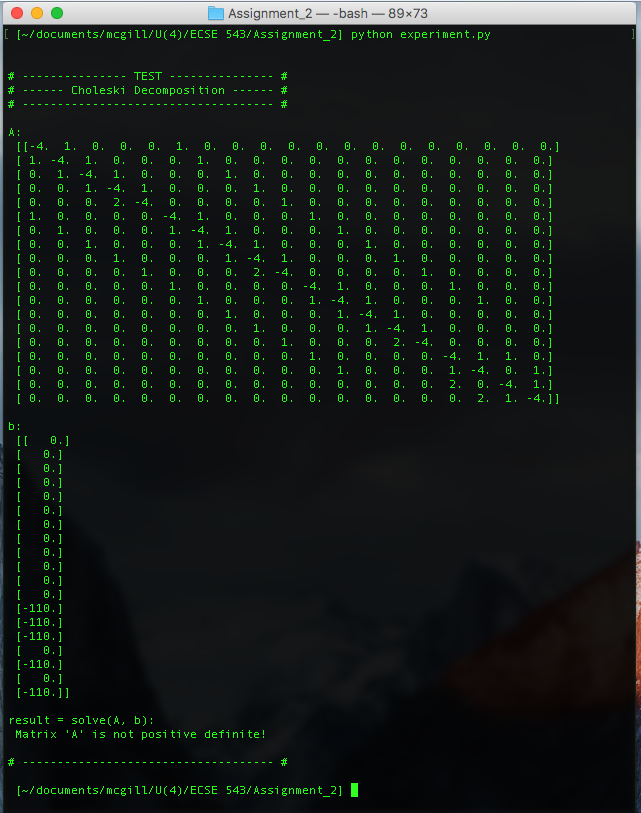
\includegraphics[width=0.7\textwidth]{assets/q3_chol}
    \caption{Console output of choleski solver used to solve the unpreconditioned finite difference equation of the bottom-left quadrant of the coax}
    \label{fig:q3_chol}
\end{figure}

\pagebreak

\subsection*{Part b}
The modified preconditioned problem is solved using the conjugate gradient method, and the choleski decomposition method. The console outputs are shown in Figures \ref{fig:q3_cg} and \ref{fig:q3_chol_II}.

\begin{figure}[h!]
    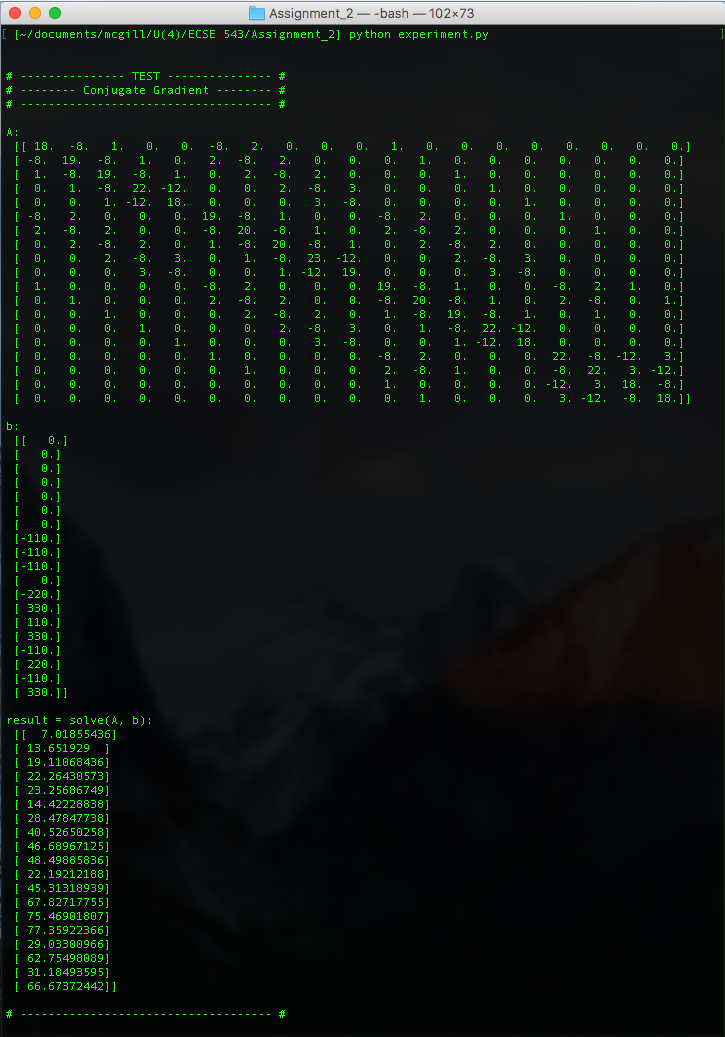
\includegraphics[width=0.7\textwidth]{assets/q3_cg}
    \caption{Console output of conjugate graident solver used to solve the preconditioned finite difference equation of the bottom-left quadrant of the coax}
    \label{fig:q3_cg}
\end{figure}
\pagebreak
\begin{figure}[h!]
    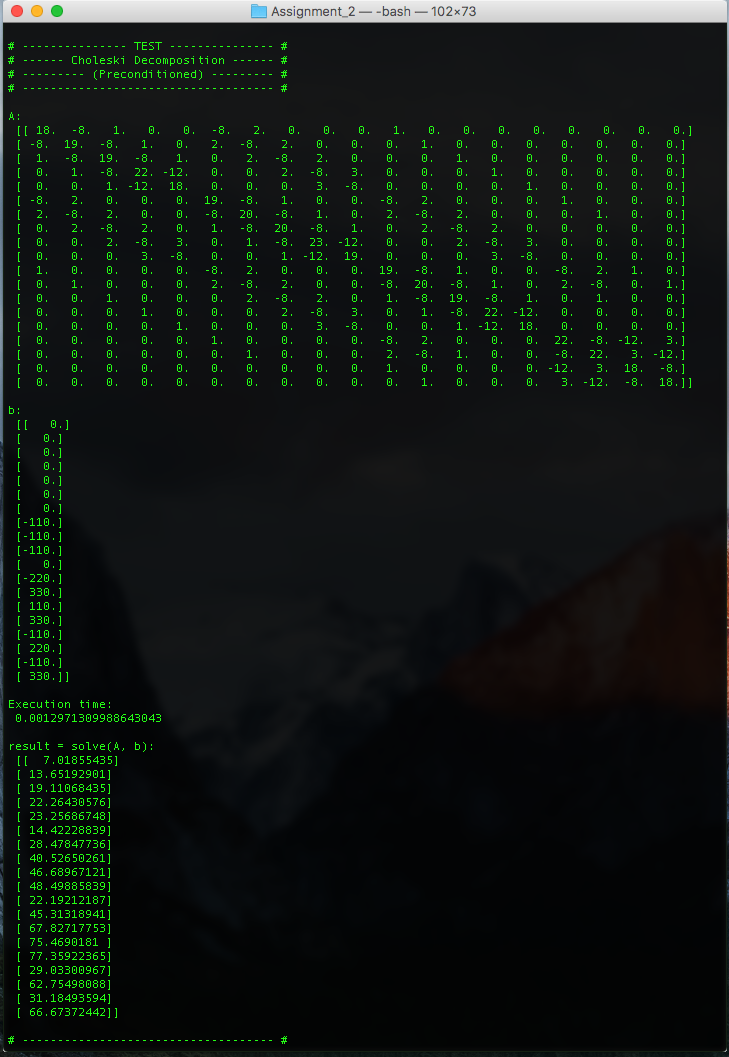
\includegraphics[width=0.7\textwidth]{assets/q3_chol_II}
    \caption{Console output of choleski solver used to solve the preconditioned finite difference equation of the bottom-left quadrant of the coax}
    \label{fig:q3_chol_II}
\end{figure}

\pagebreak

\subsection*{Part c}
A plot of the 2-norm and the infinity-norm of the residual versus iterations for the conjugate gradient program is shown below in Figure \ref{fig:q3_residual}.
\begin{figure}[h!]
   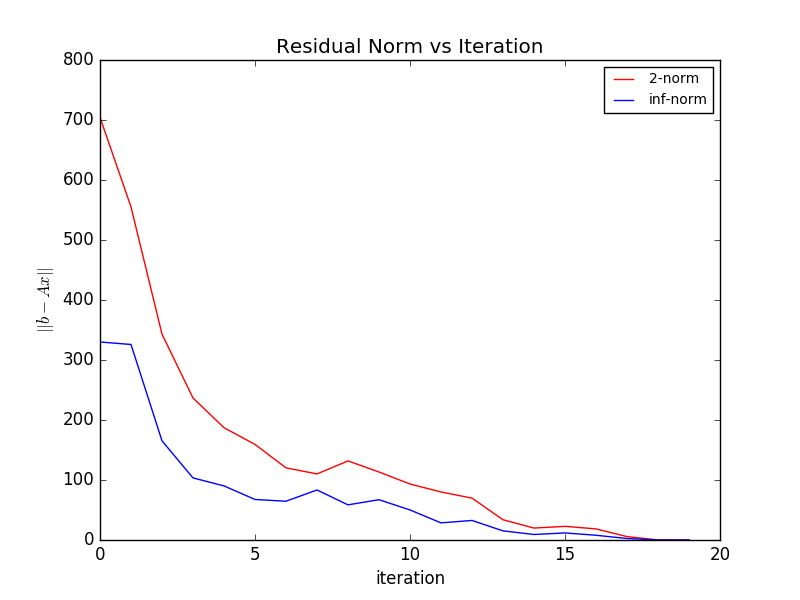
\includegraphics[width=0.8\textwidth]{assets/q3_residual}
   \caption{Plot of the 2-norm and the infinity-norm of the residual versus iterations for the conjugate gradient program.}
   \label{fig:q3_residual}
\end{figure}

\subsection*{Part d}
\textbf{The potential at (x,y) = (0.06, 0.04) is 40.52601638 Volts using the conjugate gradient method, and 40.52650261 Volts using the choleski decomposition method.} The corresponding console outputs are shown in Figures \ref{fig:cg_potential} and \ref{fig:chol_potential}. These results are very similar to the potential computed in Question 2(b), which as we recall was found to be \textbf{41.4710 Volts}. It is interesting to note that the potentials computed using conjugate gradient and choleski appears to be more accurate than that found using the SIMPLE2D program in Question 2(b). The potentials found also are very similar to the potential found at the same (x,y) location and for the same node spacing computed in Assignment 1 using SOR - which was found to be \textbf{40.5265 Volts} on aggregate spanning over the multiple different values for the parameter $\omega$. This seems to indicate that the methods that use the finite difference method all perform similarly, and perhaps more accurately than the finite element method when the finite elements are distributed as they are in Figure \ref{fig:q2_mesh}.

\begin{figure}[h!]
   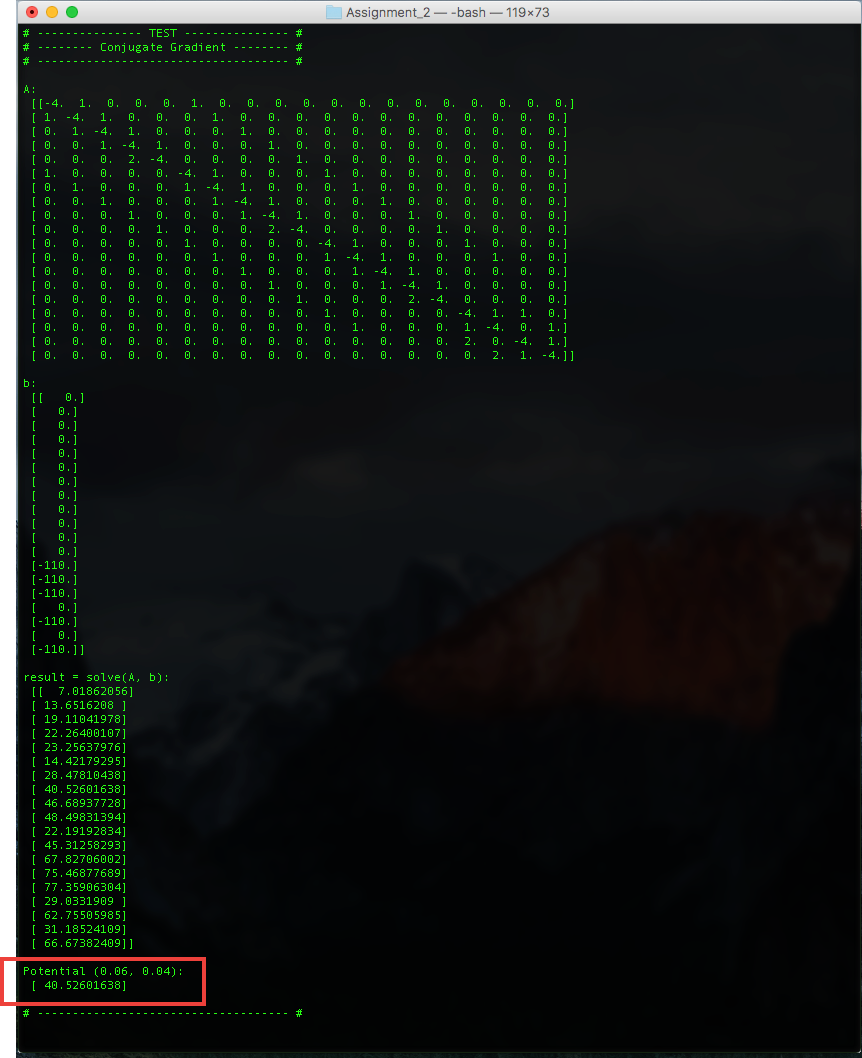
\includegraphics[width=0.95\textwidth]{assets/cg_potential}
   \caption{Console output computing the potential at (0.06, 0.04) using the conjugate gradient method}
   \label{fig:cg_potential}
\end{figure}
\pagebreak
\begin{figure}[h!]
   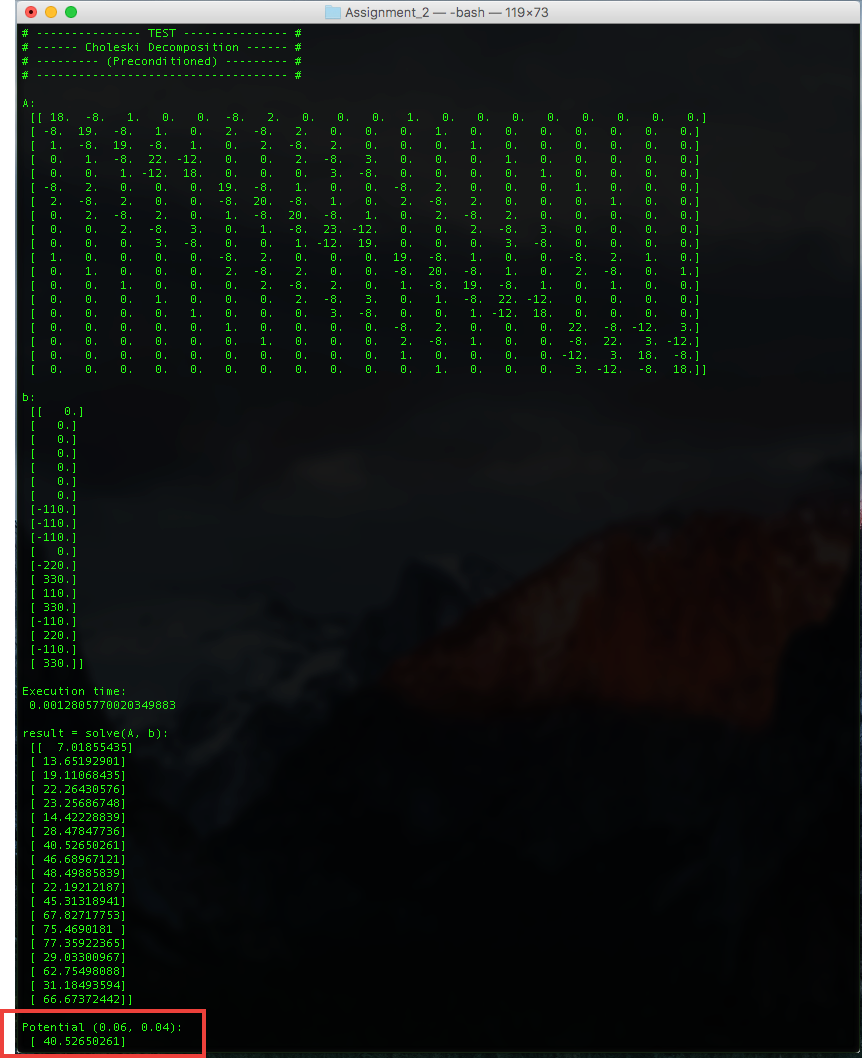
\includegraphics[width=0.95\textwidth]{assets/chol_potential}
   \caption{Console output computing the potential at (0.06, 0.04) using the choleski decomposition method}
   \label{fig:chol_potential}
\end{figure}
\pagebreak

\subsection*{Part e}
To compute the capacitance per unit length of the system from the finite difference solution, one could use a finite element energy equation, where \textbf{the vertices of the finite elements are the nodes in the finite difference mesh}. Since these potentials are known, the corresponding energies per unit length of each free potential finite element can also be determined. The energies of the individual finite elements can be subsequently added, and then one can simply used the capacitance energy equation from Question 2 to determine the capacitance per unit length of the system. Thus we have computed the capacitance per unit length from the finite difference solution.

\begin{landscape}
    \lstinputlisting[language=Python, label=lstng:experiment, frame=single, caption=experiment.py]{../experiment.py}
\end{landscape}

\begin{landscape}
    \lstinputlisting[language=Python, label=lstng:utils, frame=single, caption=utils.py]{../utils.py}
\end{landscape}

\begin{landscape}
    \lstinputlisting[language=Python, label=lstng:conjugate_gradient, frame=single, caption=conjugate\_gradient.py]{../conjugate_gradient.py}
\end{landscape}

\begin{landscape}
    \lstinputlisting[language=Python, label=lstng:choleski, frame=single, caption=choleski.py]{../choleski.py}
\end{landscape}

\begin{landscape}
    \lstinputlisting[language=Python, label=lstng:conductor, frame=single, caption=conductor\_description.py]{../conductor_description.py}
\end{landscape}



\end{document}






